

\begin{frame}{Introduction}
  \section{Introduction}
  \begin{spacing}{1.2}
  \begin{columns}[T] 
    \begin{column}{0.5\textwidth}

 \begin{itemize}
    \item The Arctic is a unique region characterized by:
    \begin{itemize}
      \item Extreme cold temperatures and vast ice sheets.
      \item Unique ecosystems and a central role in global climate systems.
    \end{itemize}
    \item Defined as the area north of the Arctic Circle ($66^{\circ}33'$ N).
    \item Two main sub-regions:
    \begin{itemize}
      \item Arctic maritime region 
      \item Arctic continental region 
    \end{itemize}
    \item Greenland is the main landmass, characterized by tundra and polar desert landscapes.
  \end{itemize}

    \end{column}
    \begin{column}{0.5\textwidth} 
      \begin{figure}
    \centering
    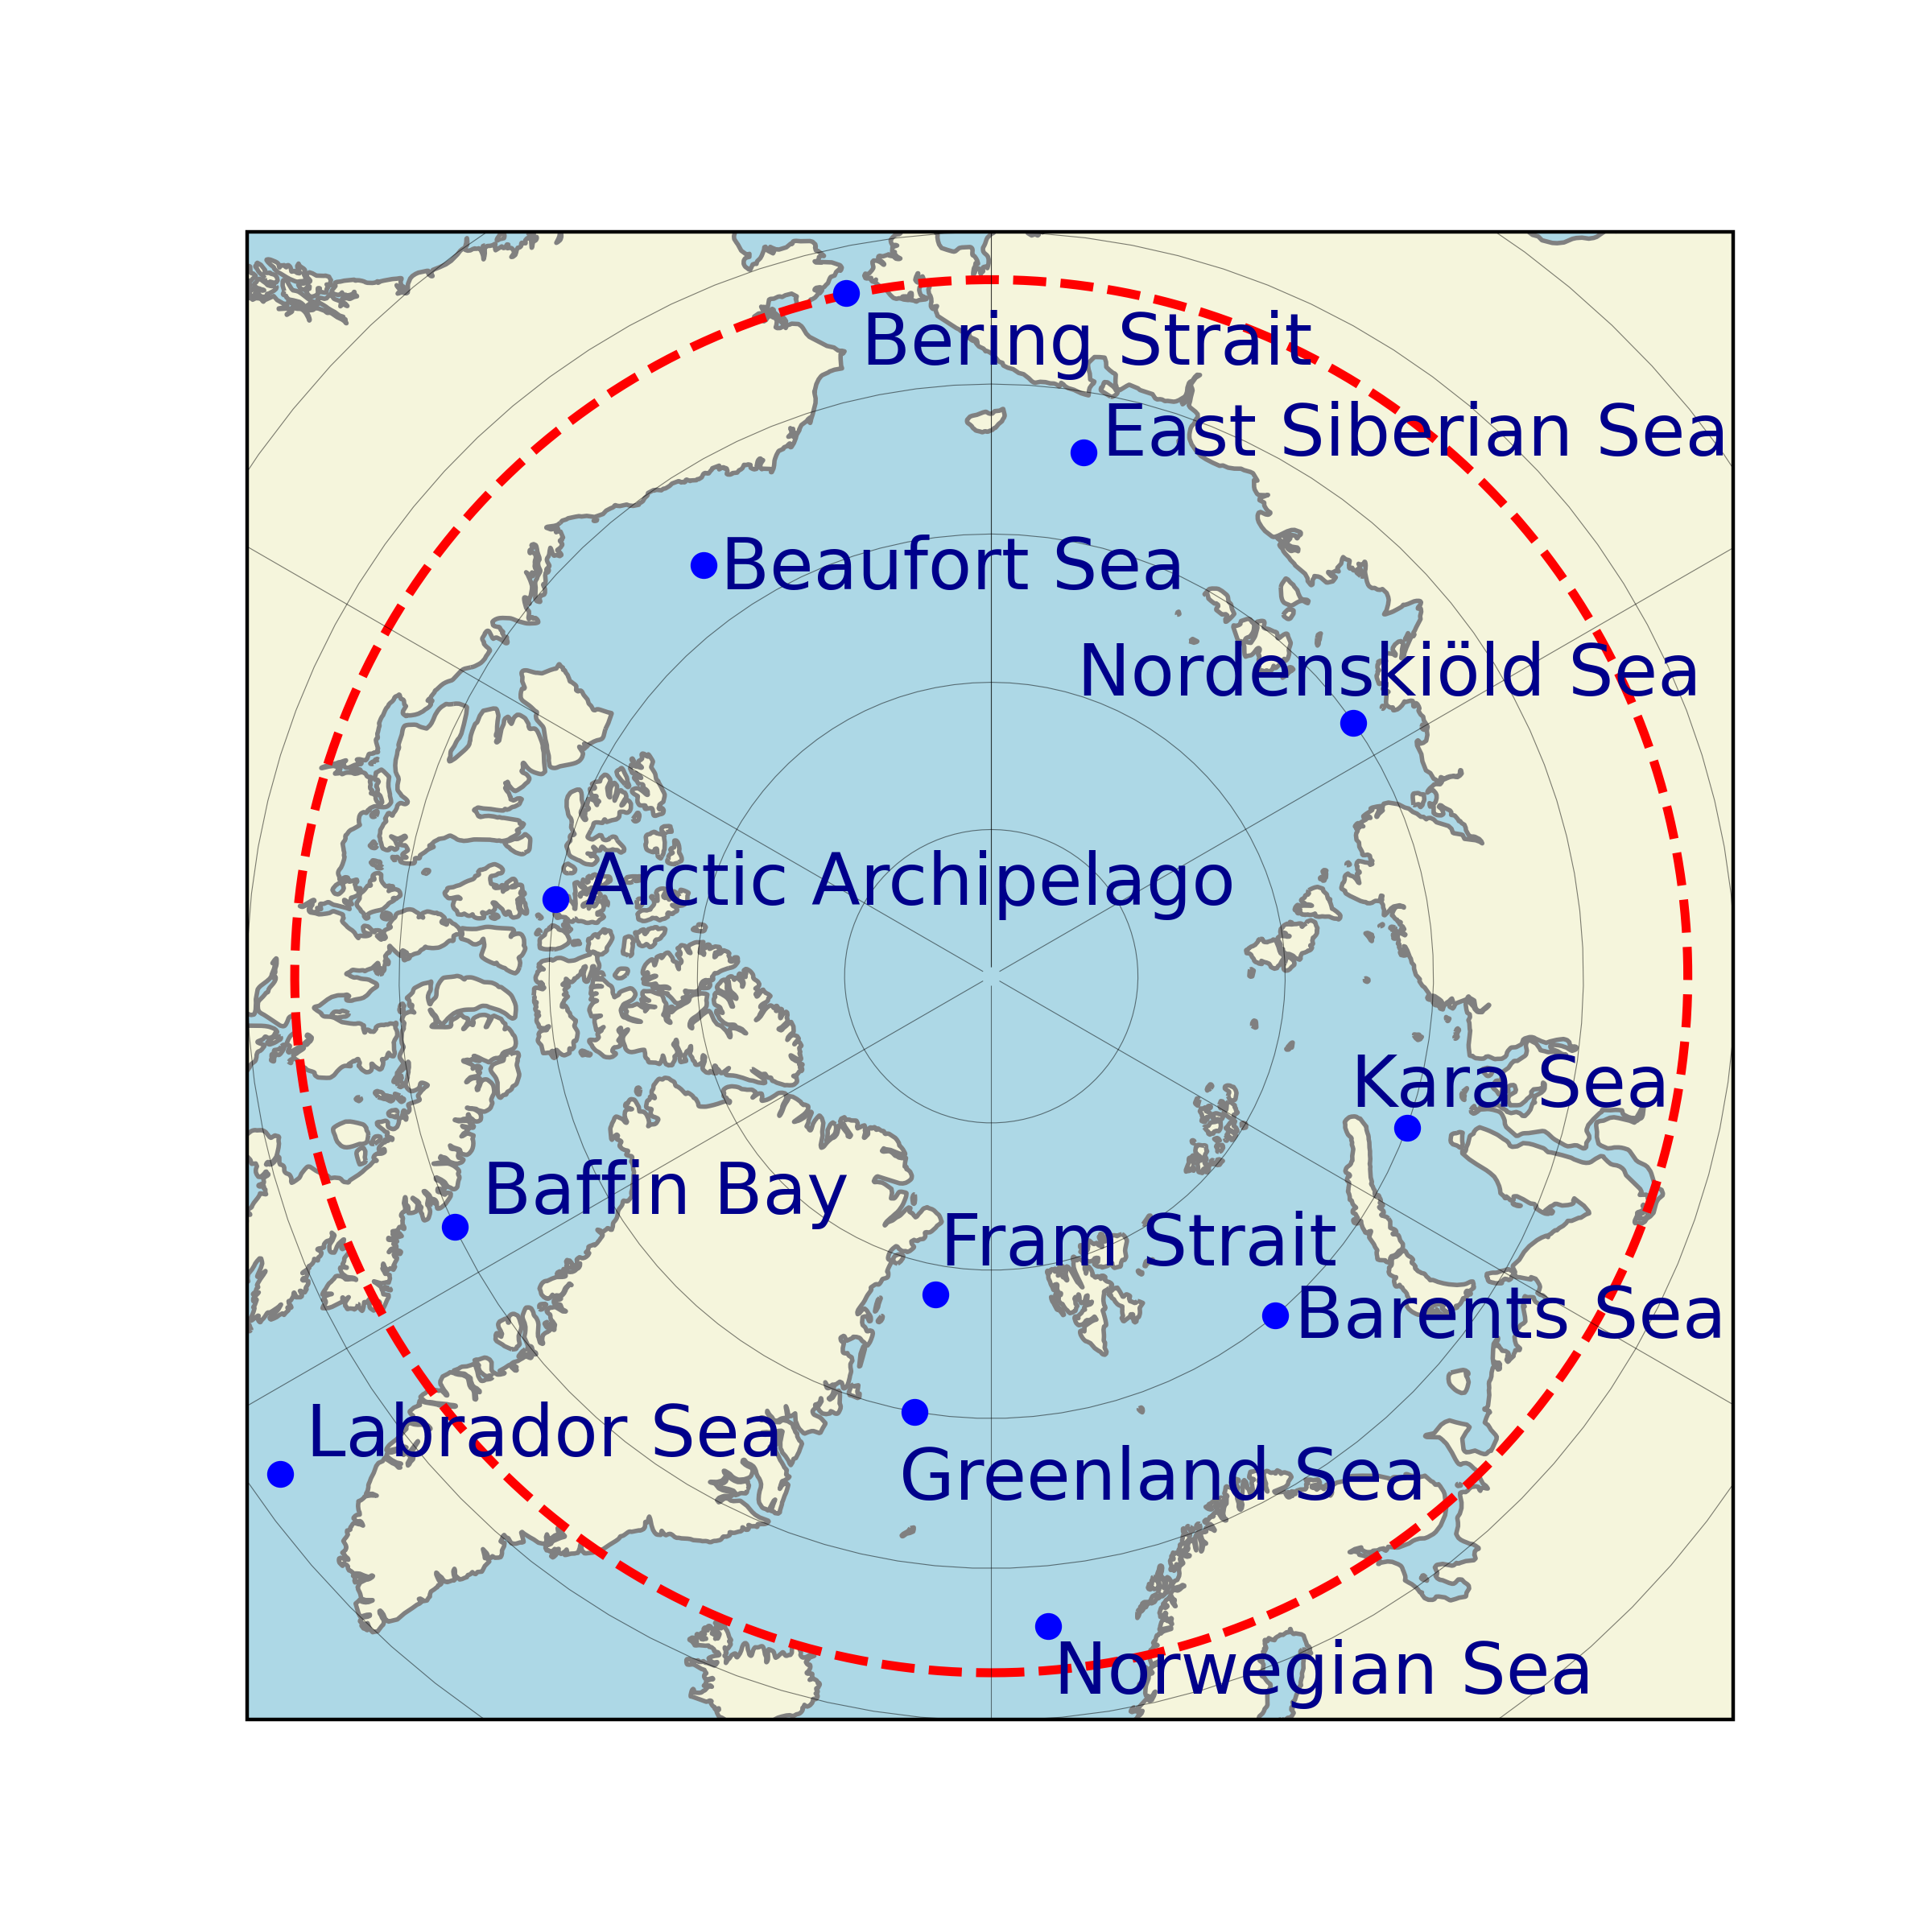
\includegraphics[width=\textwidth]{Figures/map.png}
    \caption{A map of the Arctic.}
  \end{figure}
    \end{column}
  \end{columns}
  \end{spacing}
\end{frame}



\begin{frame}{Annual Means}
    \section{The regional climate}
    \begin{figure}
        \begin{subfigure}[b]{0.49\textwidth}
            \centering
            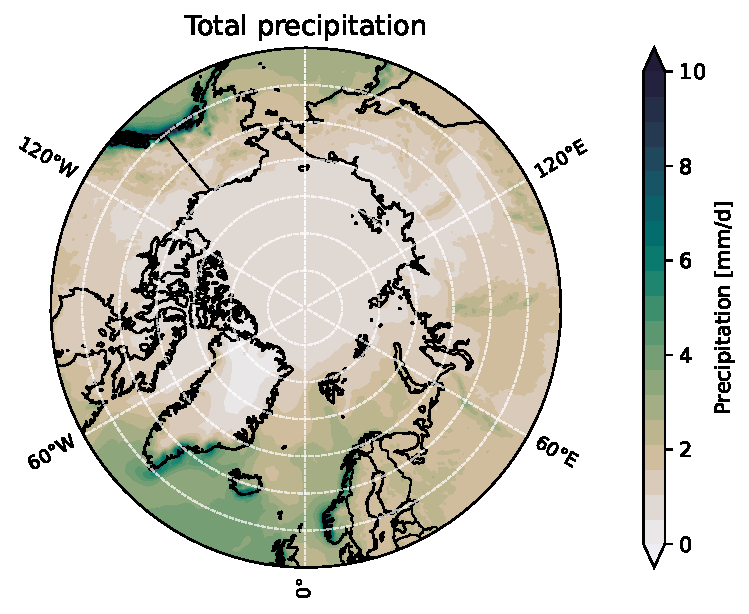
\includegraphics[height=0.4\textheight,keepaspectratio]{Figures/TotalPrecipitation_annual.pdf}
            \caption{Average daily Precipitation}
        \end{subfigure}
        \hfill
        \begin{subfigure}[b]{0.49\textwidth}
            \centering
            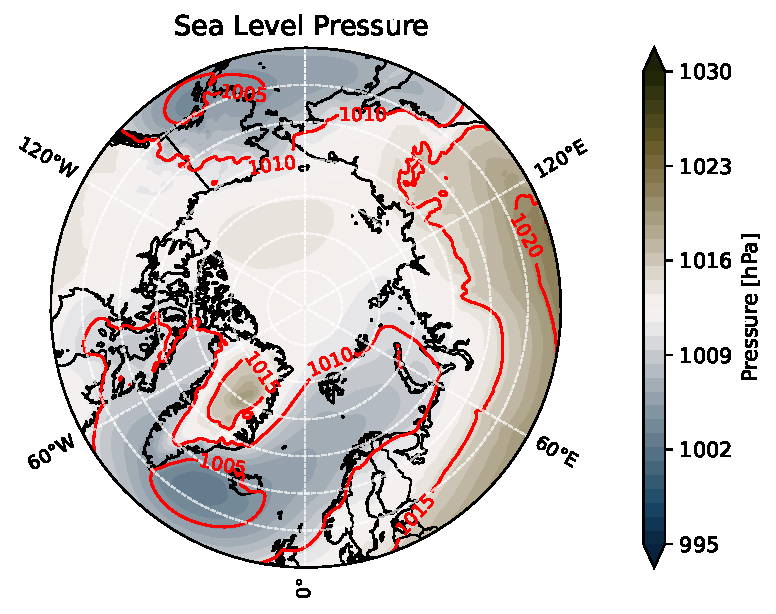
\includegraphics[height=0.4\textheight,keepaspectratio]{Figures/SeaLevelPressure_annual.pdf}
            \caption{Sea Level Pressure}
        \end{subfigure}
        \caption{Annual mean sea level pressure  and total monthly precipitation (2015--2025). All the data was downloaded through the \citet{copernicus_climate_change_service_era5_2023}.}
    \end{figure}
\end{frame}

\begin{frame}{Monthly Means}
    \begin{figure}
        \begin{subfigure}[b]{0.49\textwidth}
            \centering
            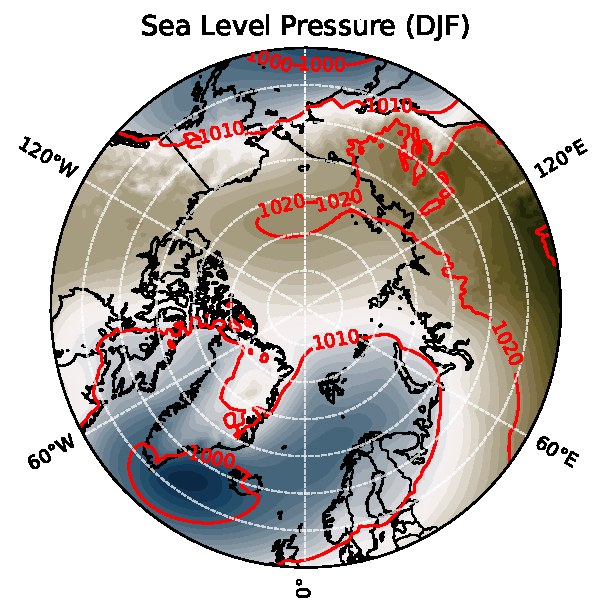
\includegraphics[height=0.4\textheight,keepaspectratio]{Figures/SeaLevelPressure_mean_DJF.pdf}
            \caption{Sea Level Pressure}
        \end{subfigure}
        \hfill
        \begin{subfigure}[b]{0.49\textwidth}
            \centering
            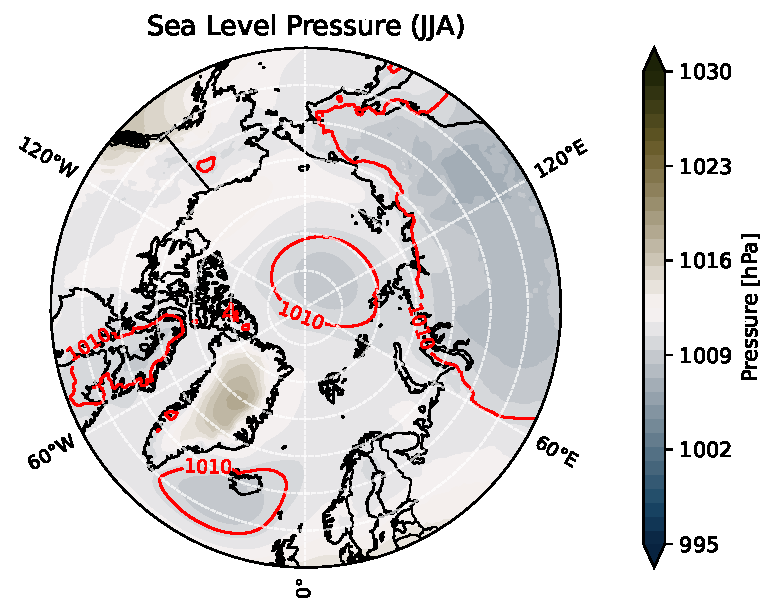
\includegraphics[height=0.4\textheight,keepaspectratio]{Figures/SeaLevelPressure_mean_JJA.pdf}
            \caption{Sea Level Pressure}
        \end{subfigure}
        \caption{Monthly mean sea level pressure  (2015--2025).}
    \end{figure}
\end{frame}

\begin{frame}{Winter conditions}
    \begin{figure}
        \begin{subfigure}[b]{0.49\textwidth}
            \centering
            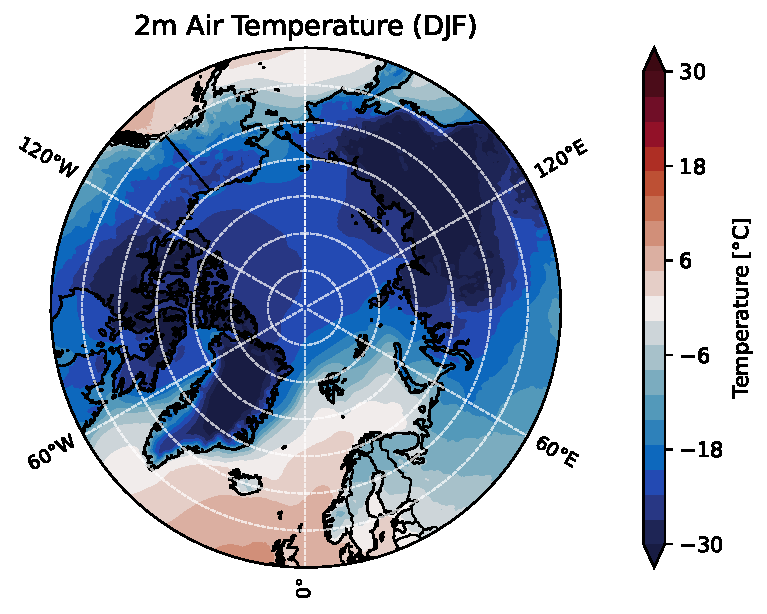
\includegraphics[height=0.4\textheight,keepaspectratio]{Figures/Temperature_mean_DJF.pdf}
            \caption{Temperature}
        \end{subfigure}
        \hfill
        \begin{subfigure}[b]{0.49\textwidth}
            \centering
            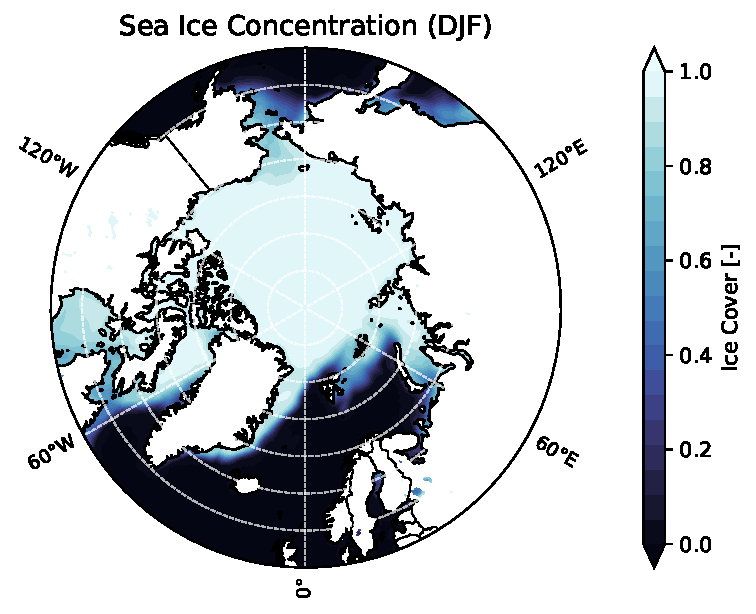
\includegraphics[height=0.4\textheight,keepaspectratio]{Figures/SeaIce_mean_DJF.pdf}
            \caption{Sea Ice}
        \end{subfigure}
    \end{figure}
\end{frame}

\begin{frame}{Spring conditions}
    \begin{figure}
        \begin{subfigure}[b]{0.49\textwidth}
            \centering
            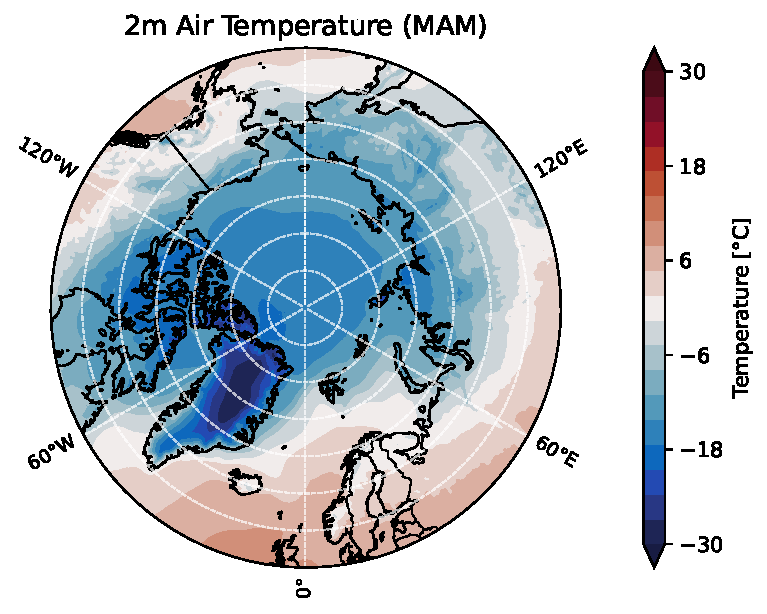
\includegraphics[height=0.4\textheight,keepaspectratio]{Figures/Temperature_mean_MAM.pdf}
            \caption{Temperature}
        \end{subfigure}
        \hfill
        \begin{subfigure}[b]{0.49\textwidth}
            \centering
            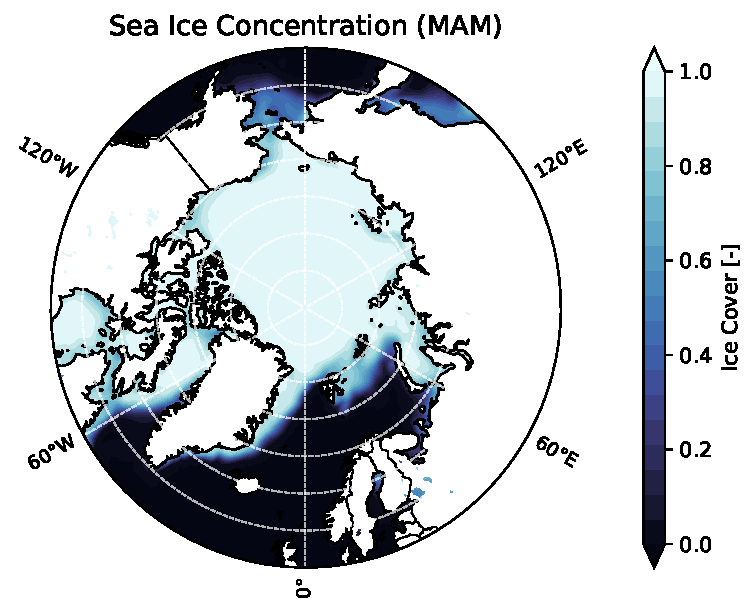
\includegraphics[height=0.4\textheight,keepaspectratio]{Figures/SeaIce_mean_MAM.pdf}
            \caption{Sea Ice}
        \end{subfigure}
    \end{figure}
\end{frame}

\begin{frame}{Summer conditions}
    \begin{figure}
        \begin{subfigure}[b]{0.49\textwidth}
            \centering
            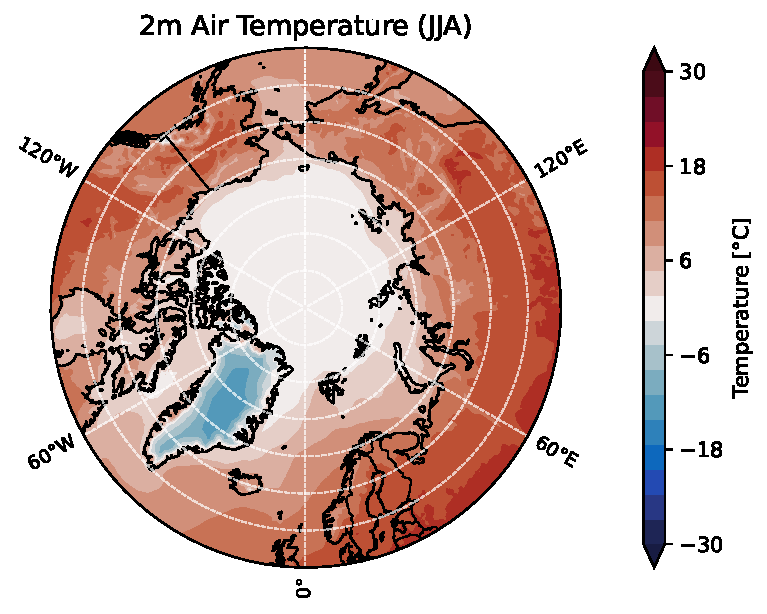
\includegraphics[height=0.4\textheight,keepaspectratio]{Figures/Temperature_mean_JJA.pdf}
            \caption{Temperature}
        \end{subfigure}
        \hfill
        \begin{subfigure}[b]{0.49\textwidth}
            \centering
            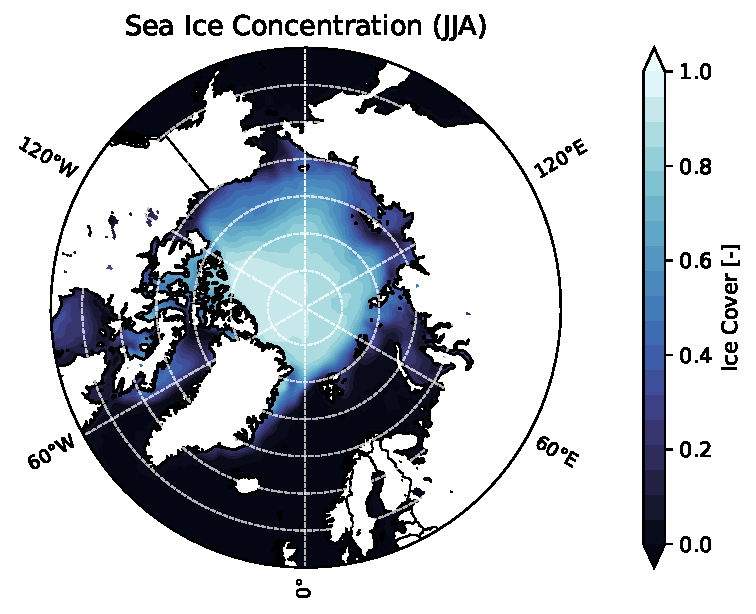
\includegraphics[height=0.4\textheight,keepaspectratio]{Figures/SeaIce_mean_JJA.pdf}
            \caption{Sea Ice}
        \end{subfigure}
    \end{figure}
\end{frame}

\begin{frame}{Autumn conditions}
    \begin{figure}
        \begin{subfigure}[b]{0.49\textwidth}
            \centering
            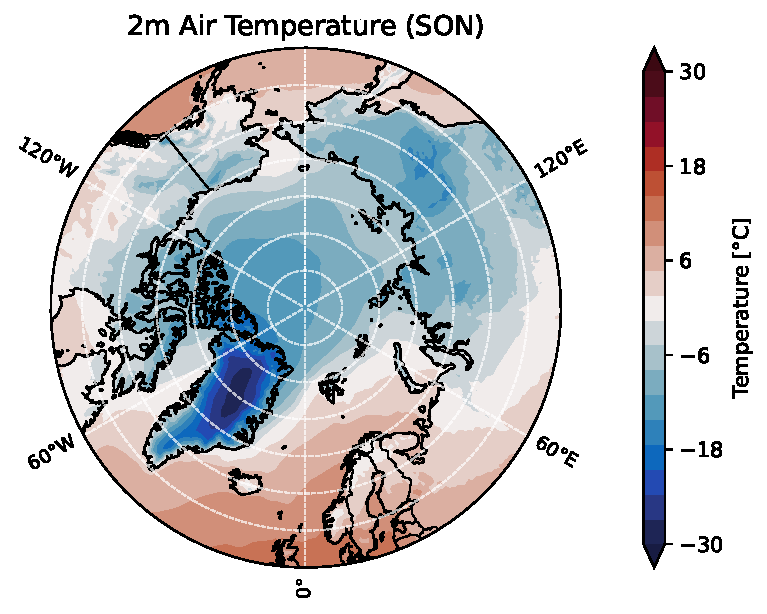
\includegraphics[height=0.4\textheight,keepaspectratio]{Figures/Temperature_mean_SON.pdf}
            \caption{Temperature}
        \end{subfigure}
        \hfill
        \begin{subfigure}[b]{0.49\textwidth}
            \centering
            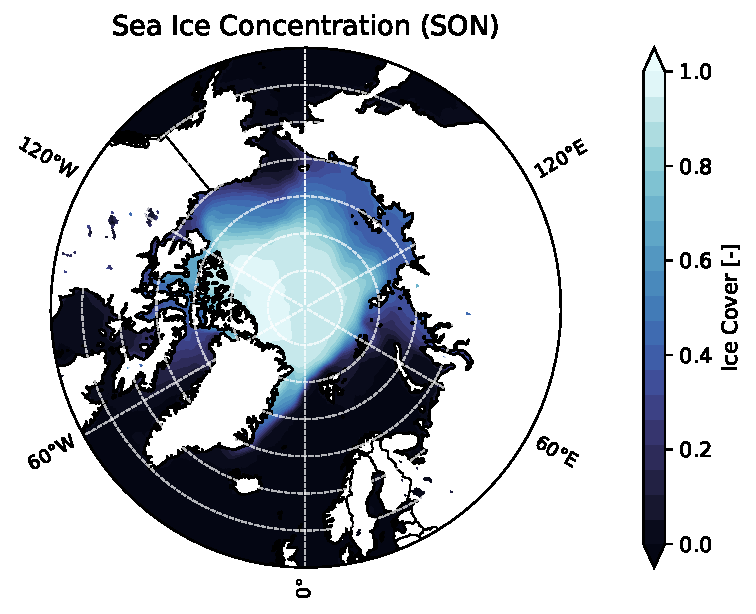
\includegraphics[height=0.4\textheight,keepaspectratio]{Figures/SeaIce_mean_SON.pdf}
            \caption{Sea Ice}
        \end{subfigure}
    \end{figure}
\end{frame}

\begin{frame}{The Atmosphere}
  \begin{spacing}{1.2} 
  \section{The general circulation}
  \begin{columns}[T] 
    \begin{column}{0.6\textwidth} 

\begin{itemize}
    \item The Arctic atmosphere is influenced by large-scale circulation patterns:
    \begin{itemize}
      \item Hadley, Ferrel, and Polar cells.
      \item Polar cell subsidizes air in the North Pole, creating a high-pressure system.
    \end{itemize}
    \item Key features:
    \begin{itemize}
      \item Dry, desert-like climate due to subsidence of cold air together with inversion.
      \item Southerly winds drive water southward.
      \item Arctic Oscillation (AO) measures pressure differences between the Arctic and mid-latitudes.
    \end{itemize}
    \item Seasonal variability:
    \begin{itemize}
      \item Stronger AO during winter due to temperature gradients.
      \item Extratropical cyclones are common in winter near the Icelandic and Aleutian lows \citep{serreze2014}.
    \end{itemize}
  \end{itemize}

    \end{column}
    \begin{column}{0.4\textwidth} 
      \begin{figure}
        \centering
        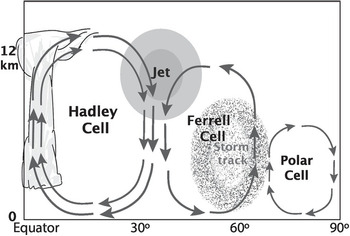
\includegraphics[width=0.8\textwidth]{Figures/polar-cell.jpg}
        \caption{The polar cell illustrated \citep{Trenberth_2022}}
      \end{figure}
      \begin{figure}
        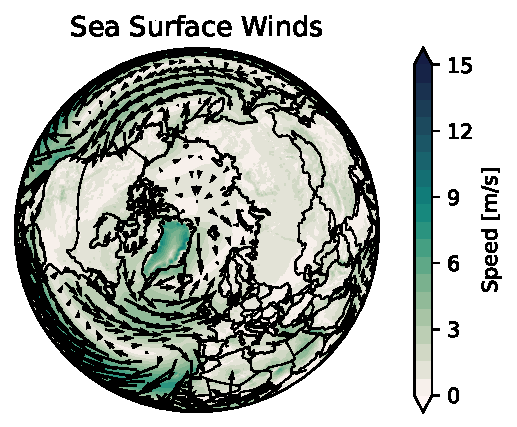
\includegraphics[width=0.8\textwidth]{Figures/SurfaceWind_annual.pdf}
        \caption{Surface winds (2015--2025)}
      \end{figure}
    \end{column}
  \end{columns}
  \end{spacing}
\end{frame}


\begin{frame}{The Ocean}
  \begin{spacing}{1.2} 
  \begin{columns}[T] 
    \begin{column}{0.6\textwidth} 
      \begin{itemize}

    \item The Arctic Ocean is semi-isolated, connected to the Atlantic through the Fram Strait.
    \item Arctic part of the global meridional overturning circulation:
    \begin{itemize}
      \item Norwegian Current brings warm, saline water into the Arctic.
      \item Heat flux from ocean to atmosphere as water cools and freezes.
      \item Brine rejection increases salinity and density, causing water to sink.
      \item Water exits as cold, less saline North Atlantic Deep Water (NADW).
    \end{itemize}
    \item Transport and river discharge contribute to southward flow through the East Greenland and Labrador Currents.
    \item Sea ice outflow through Beaufort Gyre and transpolar drift. 

    
  \end{itemize}
    \end{column}
    \begin{column}{0.4\textwidth} 
      \begin{figure}
        \centering
        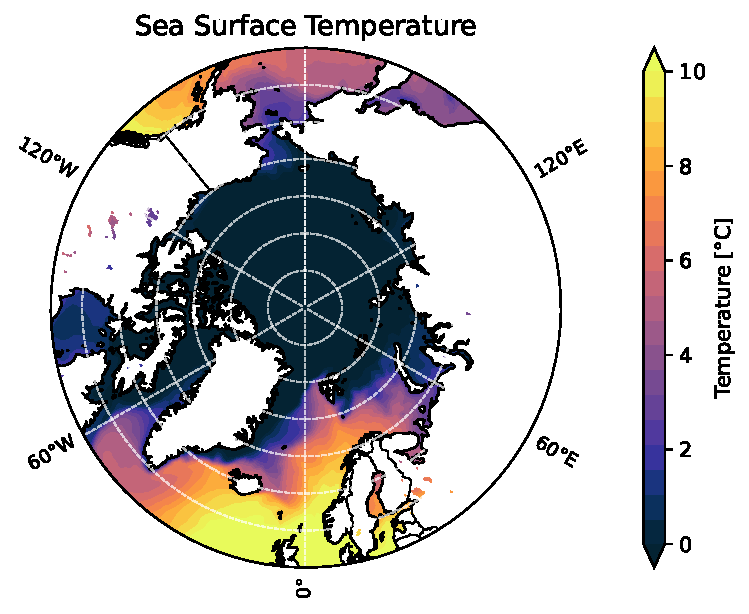
\includegraphics[width=\textwidth]{Figures/SeaSurfaceTemperature_annual.pdf}
        \caption{Sea Surface Temperature (2015--2025)}
      \end{figure}
    \end{column}
  \end{columns}
  \end{spacing}
\end{frame}




\begin{frame}{Climate Change}
    \section{Climate Change}
    \begin{spacing}{1.5} 
\begin{itemize}

    \item The Arctic is warming at nearly four times the global average rate (Arctic amplification) \citep{rantanen2022}.
    \item Key impacts:
    \begin{itemize}
      \item Decline in sea ice extent, reducing albedo and increasing solar absorption.
      \item Thawing permafrost releases greenhouse gases, further enhancing warming.
      \item Changes in river flow patterns and landscape due to thawing.
    \end{itemize}
    \item Projected future changes:
    \begin{itemize}
      \item Arctic Ocean may be ice-free during summer by 2050 \citep{hartmann2016}.
      \item Significant impacts on ecosystems and Indigenous communities.
    \end{itemize}

  \end{itemize}
  \end{spacing}
\end{frame}


\begin{frame}{Societal activities}
    \section{Societal activities}
    \begin{spacing}{1.5} 
  \begin{itemize}

    \item Climate change impacts on societal activities:
    \begin{itemize}
      \item Opening of new shipping routes due to sea ice retreat.
      \item Increased interest in resource extraction (minerals, oil).
    \end{itemize}
    \item Geopolitical implications:
    \begin{itemize}
      \item Growing interest from major powers (e.g., the United States) in controlling Arctic routes and resources \citep{CongressionalResearchService2026}.
      \item Potential impacts on Indigenous peoples and the Arctic environment according to \citet{IPCC2023}.
    \end{itemize}

  \end{itemize}
  \end{spacing}
\end{frame}